%# -*- coding:utf-8 -*-
\chapter{符号说明与预备知识}\label{chap:prelim}
\echapter{Notations and Preliminaries}
本章将首先介绍本文中使用到的符号,而后将介绍一些必要的预备知识。

\section{符号说明}\label{sec:notation}
\esection{Notations}
本节介绍本文中使用到的符号。总体来讲,本文使用粗体书法体字母来代表张量(如$\mathbfcal{X}$),粗体大写字母来代表矩阵(如$\boldsymbol{X}$),粗体小写字母来代表向量(如$\boldsymbol{x}$),而一般的小写字母来代表标量(如$x$)。对于向量$\boldsymbol{x}$,矩阵$\boldsymbol{X}$,张量$\mathbfcal{X}$,它们的某个元素分别被表示为$x_{i}$,$x_{i j}$或$x_{i j k}$。此外,为了表述方便,有时也使用$(\boldsymbol{X})_{i j}$来代表矩阵$\boldsymbol{X}$的元素。本节接下来分别对向量/矩阵相关的符号以及张量相关的符号进行介绍。

\begin{table}[!b]
% \captionsetup{labelsep=newline}
\centering
\caption{向量/矩阵相关的符号总结}
\label{tab:matrix-notations}
\begin{tabular}{l|l|l|l}
\hline
$\boldsymbol{x}$ & 向量 & $\boldsymbol{X}$ & 矩阵 \\
$\boldsymbol{x}_{i:}$,$\boldsymbol{x}_{:j}$ & $\boldsymbol{X}$的第$i$行和第$j$列 & $\operatorname{rank}(\boldsymbol{X})$ & $\boldsymbol{X}$的秩 \\
$\operatorname{Tr}(\boldsymbol{X})$ & $\boldsymbol{X}$的迹 & $\boldsymbol{X}^{\top}$ & $\boldsymbol{X}$的转置 \\
$\norm{\boldsymbol{X}}_F$ & $\boldsymbol{X}$的Frobenius范数 & $\norm{\boldsymbol{X}}_{2,1}$ & $\boldsymbol{X}$的$\ell_{2,1}$范数 \\ $(\boldsymbol{X})_{+}$ & $\boldsymbol{X}$的正部 & $\boldsymbol{I}_{n}$ & $n\times n$的单位矩阵 \\
$\boldsymbol{I}_{m,n}$ & $m\times n$的单位矩阵 & $\boldsymbol{0}_{m,n}$ & $m\times n$的全$0$矩阵 \\ $\boldsymbol{1}_{n}$ & $n$维全$1$向量 & $\operatorname{diag}(\boldsymbol{x})$ & $\boldsymbol{x}$作为对角线的对角矩阵 \\
$\operatorname{vec}^{-1}_{m,n}(\boldsymbol{x})$ & $\boldsymbol{x}$的逆向量化 & $\operatorname{vec}(\boldsymbol{X})$ & $\boldsymbol{X}$的向量化 \\\hline
$\otimes$ & Kronecker积 & $\odot$ & Khatri-Rao积 \\ $\oast$ & Hadamard积 & $\oslash$或$/$& 两个矩阵之间逐元素的除法 \\ \hline
\end{tabular}
% \vspace{-2em}
\end{table}

% \subsection{矩阵相关的符号}
% \esubsection{Notations Related to Matrices}
% 在本小节,我们介绍矩阵相关的符号。
对矩阵$\boldsymbol{X}\in\mathbb{R}^{n_1\times n_2}$而言,$\boldsymbol{x}_{i:}$和$\boldsymbol{x}_{:j}$分别代表该矩阵的第$i$行和第$j$列。$\operatorname{rank}(\boldsymbol{X})$代表矩阵$\boldsymbol{X}$的秩。此外,如果矩阵$\boldsymbol{X}$是方阵,则$\operatorname{Tr}(\boldsymbol{X})$表示它的迹。$\boldsymbol{X}^{\top}$代表矩阵$\boldsymbol{X}$的转置,$\norm{\boldsymbol{X}}_F$表示矩阵$\boldsymbol{X}$的Frobenius范数。$\otimes$表示两个矩阵之间的Kronecker积,$\odot$表示两个矩阵之间的Khatri-Rao积,$\oast$表示两个矩阵之间逐元素的乘法(或Hadamard积),而$\oslash$或$/$表示两个矩阵之间逐元素的除法
% \footnote{对于两个同样大小的矩阵$\boldsymbol{X}$和$\boldsymbol{Y}$,有时也使用${\boldsymbol{X}}/{\boldsymbol{Y}}$来表示它们之间的逐元素的除法。}
。除此之外,矩阵$\boldsymbol{X}$的$\ell_{2,1}$范数被表示为$\norm{\boldsymbol{X}}_{2,1}:=\sum_{i=1}^{n_1} \sqrt{\sum_{j=1}^{n_2} x_{i j}^{2}}$,而$\boldsymbol{X}$的正部被表示为$(\boldsymbol{X})_{+}$。$\boldsymbol{I}_{n}$代表$n\times n$的单位矩阵,$\boldsymbol{I}_{m,n}$代表$m\times n$的单位矩阵(其可以被想象为足够大的单位阵的左上$m\times n$子矩阵),$\boldsymbol{0}_{m,n}$代表$m\times n$的全$0$矩阵,而$\boldsymbol{1}_{n}$代表$n$维全$1$向量。$\operatorname{diag}(\boldsymbol{x})$表示由$\boldsymbol{x}$作为对角元素(并保留$\boldsymbol{x}$中元素顺序)的对角矩阵。$\operatorname{vec}(\boldsymbol{X})$表示矩阵$\boldsymbol{X}$的向量化,即将矩阵$\boldsymbol{X}$的列向量按索引增长顺序进行拼接得到的$n_{1}n_{2}$维向量,而$\operatorname{vec}^{-1}_{m,n}(\boldsymbol{x})$表示向量$\boldsymbol{x}$的逆向量化,即将向量$\boldsymbol{x}$按照索引增长顺序逐列填充$m\times n$的矩阵得到的结果。为了方便查阅,这些符号的定义被归纳在\reftab{tab:matrix-notations}中。本节接下来给出Kronecker积、Khatri-Rao积、逐元素乘除法以及逆向量化的具体定义。

\begin{definition}[Kronecker积]\kaishu
	给定两个矩阵$\boldsymbol{A}\in\mathbb{R}^{m\times n}$和$\boldsymbol{B}\in\mathbb{R}^{p\times q}$,则它们之间的Kronecker积为
	\begin{equation*}
		\boldsymbol{A} \otimes \boldsymbol{B}:=\left[\begin{array}{cccc}
		a_{11} \boldsymbol{B} & a_{12} \boldsymbol{B} & \cdots & a_{1 n} \boldsymbol{B} \\
		a_{21} \boldsymbol{B} & a_{22} \boldsymbol{B} & \cdots & a_{2 n} \boldsymbol{B} \\
		\vdots & \vdots & \ddots & \vdots \\
		a_{m 1} \boldsymbol{B} & a_{m 2} \boldsymbol{B} & \cdots & a_{m n} \boldsymbol{B}
		\end{array}\right]\in\mathbb{R}^{mp\times nq}.
	\end{equation*}
\end{definition}

\begin{definition}[Khatri-Rao积]\kaishu
	给定两个矩阵$\boldsymbol{A}\in\mathbb{R}^{m\times n}$和$\boldsymbol{B}\in\mathbb{R}^{p\times n}$,则它们之间的Khatri-Rao积为
	\begin{equation*}
		\boldsymbol{A} \odot \boldsymbol{B}:=\left[\begin{array}{cccc}
		\boldsymbol{a}_{:1}\otimes\boldsymbol{b}_{:1} & \boldsymbol{a}_{:2}\otimes\boldsymbol{b}_{:2} & \cdots & \boldsymbol{a}_{:n}\otimes\boldsymbol{b}_{:n}
		\end{array}\right]\in\mathbb{R}^{mp\times n}.
	\end{equation*}
\end{definition}

% 我们将会在后续的张量分解章节看到,Kronecker积与Khatri-Rao积能为各种张量分解的矩阵化提供巨大的帮助。

\begin{definition}[逐元素乘法]\kaishu
	给定两个矩阵$\boldsymbol{A}\in\mathbb{R}^{m\times n}$和$\boldsymbol{B}\in\mathbb{R}^{m\times n}$,则它们之间的逐元素乘法为
	\begin{equation*}
		\boldsymbol{A} \oast \boldsymbol{B}:=\left[\begin{array}{cccc}
			a_{11}b_{11} & a_{12}b_{12} & \cdots & a_{1 n}b_{1 n} \\
			a_{21}b_{21} & a_{22}b_{22} & \cdots & a_{2 n}b_{2 n} \\
			\vdots & \vdots & \ddots & \vdots \\
			a_{m 1}b_{m 1} & a_{m 2}b_{m 2} & \cdots & a_{m n}b_{m n}
		\end{array}\right]\in\mathbb{R}^{m\times n}.
	\end{equation*}
\end{definition}

\begin{definition}[逐元素除法]\kaishu
	给定两个矩阵$\boldsymbol{A}\in\mathbb{R}^{m\times n}$和$\boldsymbol{B}\in\mathbb{R}^{m\times n}$,则它们之间的逐元素除法为
	\begin{equation*}
		\boldsymbol{A} \oslash \boldsymbol{B}=\frac{\boldsymbol{A}}{\boldsymbol{B}}:=\left[\begin{array}{cccc}
		a_{11}/b_{11} & a_{12}/b_{12} & \cdots & a_{1 n}/b_{1 n} \\
		a_{21}/b_{21} & a_{22}/b_{22} & \cdots & a_{2 n}/b_{2 n} \\
		\vdots & \vdots & \ddots & \vdots \\
		a_{m 1}/b_{m 1} & a_{m 2}/b_{m 2} & \cdots & a_{m n}/b_{m n}
		\end{array}\right]\in\mathbb{R}^{m\times n}.
	\end{equation*}
\end{definition}

% 本节接下来定义矩阵的逆向量化。

\begin{definition}[逆向量化]\kaishu
	定义映射$\operatorname{vec}^{-1}_{m,n}:\mathbb{R}^{mn}\rightarrow\mathbb{R}^{m\times n}$,
	\begin{equation*}
		\operatorname{vec}^{-1}_{m,n}(\boldsymbol{x}) := \left(\left(\operatorname{vec}\left(\boldsymbol{I}_{n}\right)\right)^{\top} \otimes \boldsymbol{I}_{m}\right)(\boldsymbol{I}_{n} \otimes \boldsymbol{x}).
	\end{equation*}
% 	为从向量空间$\mathbb{R}^{mn}$到向量空间$\mathbb{R}^{m\times n}$的逆向量化映射。
\end{definition}

直观上来讲,$\operatorname{vec}^{-1}_{m,n}(\boldsymbol{x})$保留了向量$\boldsymbol{x}$中元素在列方向上的顺序。

\begin{example}\kaishu
	例如,对向量$\boldsymbol{x}_{0}=[1,2,3,4,5,6,7,8]^{\top}\in\mathbb{R}^{8}$而言,它的逆向量化$$\operatorname{vec}^{-1}_{2,4}(\boldsymbol{x}_{0}) = \begin{bmatrix}1 & 3 & 5 & 7\\2 & 4 & 6 & 8\end{bmatrix} \in \mathbb{R}^{2\times 4}.$$
\end{example}

% \subsection{张量相关的符号}
% \esubsection{Notations Related to Tensors}
% 在本小节,我们介绍张量相关的符号。
对$d$阶张量$\mathbfcal{X}\in\mathbb{R}^{n_1\times n_2\times \ldots \times n_{d}}$而言,固定所有除第$i$个索引以外的所有索引所得到的向量被称为$\mathbfcal{X}$的mode-$i$纤维。类似地,固定所有除第$i$和$j$个索引以外的所有索引所得到的矩阵被称为$\mathbfcal{X}$的mode-$(i,j)$切片。$\boldsymbol{X}_{(i)}$代表张量$\mathbfcal{X}$沿着第$i$个mode的矩阵化(其列向量由张量$\mathbfcal{X}$的mode-$i$纤维按索引增长顺序排列而成)。$\mathbfcal{X} \times_{i} \boldsymbol{U}$代表张量$\mathbfcal{X}$与矩阵$\boldsymbol{U}$的mode-$i$积。与矩阵类似,$\norm{\mathbfcal{X}}_{F}$表示张量$\mathbfcal{X}$的Frobenius范数。如果$\mathbfcal{X}$可以被表示成$d$个向量的外积,则称$\mathbfcal{X}$为秩-$1$张量。
% 我们定义张量$\mathbfcal{X}$的$k$-秩$\operatorname{rank}_{k}(\mathbfcal{X})$为矩阵$\boldsymbol{X}_{(k)}$的秩($k=1,2,\ldots,d$),并且我们称张量$\mathbfcal{X}$为$\operatorname{rank}-(r_1,r_2, \ldots ,r_d)$张量,如果$\operatorname{rank}_{k}(\mathbfcal{X})=r_{k},~\forall~k=1,2,\ldots,d$。
此外,对三阶张量$\mathbfcal{X}\in\mathbb{R}^{n_1\times n_2\times n_3}$而言,$\boldsymbol{X}_{::i}$或$\boldsymbol{X}^{(i)}$交替地代表张量$\mathbfcal{X}$的第$i$个前向切片,而$\boldsymbol{x}_{ij:}$代表张量$\mathbfcal{X}$的第$(i,j)$个mode-$3$纤维。
对于这些张量符号的详细数学定义以及细节,本文推荐读者阅读综述文章\ucite{kolda2006multilinear,kolda2009tensor}。除上述符号外,本文还定义了一种新的张量运算符$\mydiag(\cdot)$,其旨在为三阶张量提取“对角”元素。直观上来讲,类似于将方阵的对角线元素提取出构成向量的操作,$\mydiag(\cdot)$将三阶张量的“对角”元素提取出构成矩阵。为了方便查阅,这些符号的定义被归纳在\reftab{tab:tensor-notations}中。本节接下来给出$\mydiag(\cdot)$的具体定义。

\begin{definition}[三阶张量“对角”元素]\kaishu
	定义映射$\mydiag:\mathbb{R}^{j\times j\times k}\rightarrow\mathbb{R}^{j\times k}$,
	\begin{equation*}
		\mydiag(\mathbfcal{Y}):=\begin{bmatrix}\boldsymbol{y}_{11:}^{\top}\\\boldsymbol{y}_{22:}^{\top}\\\vdots\\\boldsymbol{y}_{jj:}^{\top}\end{bmatrix}=\begin{bmatrix}y_{1 1 1}&y_{1 1 2}&\ldots&y_{1 1 k}\\y_{2 2 1}&y_{2 2 2}&\ldots&y_{2 2 k}\\\vdots&\vdots&\ddots&\vdots\\y_{j j 1}&y_{j j 2}&\ldots&y_{j j k}\end{bmatrix}.
	\end{equation*}

	% \reffig{fig:diag3}形象地展示了$\mydiag$的功能。
	
	% \begin{figure}[!ht]
	%   \centering
	%   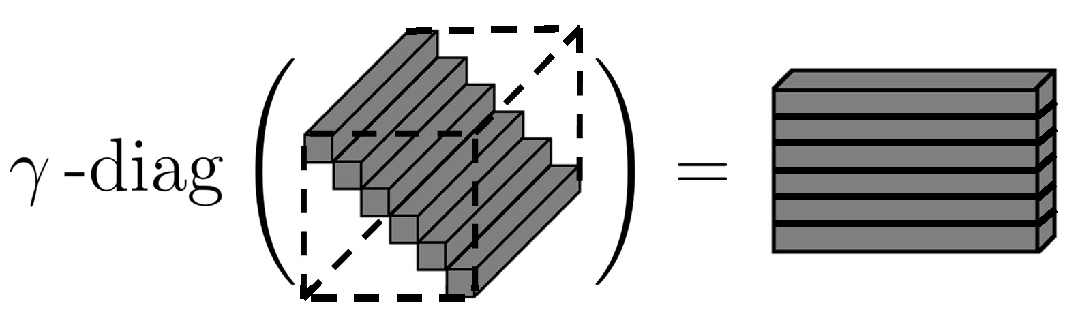
\includegraphics[width=.75\linewidth]{figures/diag3.pdf}
	%   \captionsetup{labelsep=period,justification=justified,singlelinecheck=false}
	%   \caption{$\mydiag$的一个形象展示}
	%   \label{fig:diag3}
	% \end{figure}
\end{definition}

\noindent 对于定义在$\mathbb{R}^{j\times j\times k}$中的三阶张量$\mathbfcal{Y}$,$\mydiag(\mathbfcal{Y}) \in \mathbb{R}^{j\times k}$即代表$\mathbfcal{Y}$的“对角”元素,其行向量由$\mathbfcal{Y}$的前两个索引相同的mode-$3$纤维(即$\{\boldsymbol{y}_{ii:}\}_{i=1}^{j}$)组成。\reffig{fig:diag3}形象地展示了$\mydiag(\cdot)$的作用。

\begin{figure}[!ht]
	  \centering
	  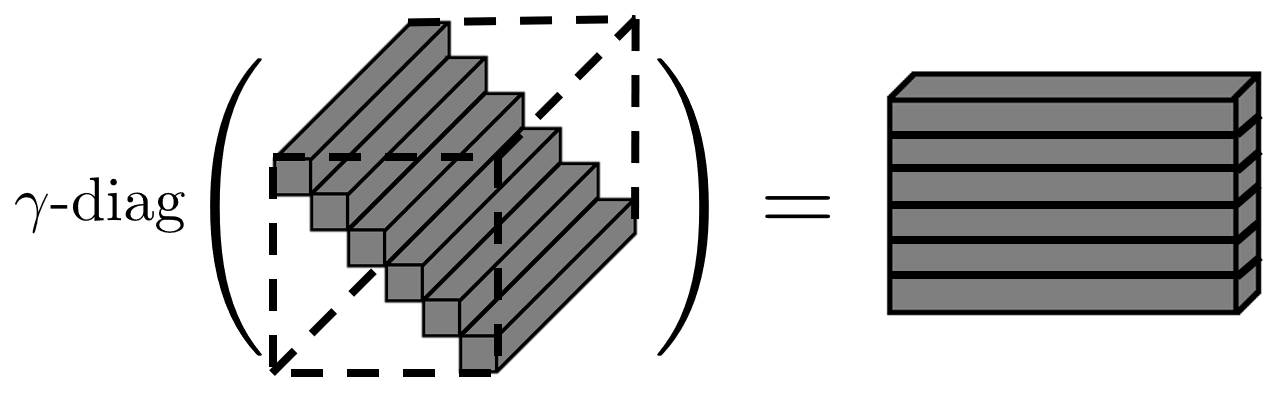
\includegraphics[width=.7\linewidth]{figures/gammadiag.png}
	  \caption{$\mydiag(\cdot)$的示意图}
	  \label{fig:diag3}
\end{figure}

\begin{table}[!t]
% \captionsetup{labelsep=newline}
\centering
\caption{张量相关的符号总结}
\label{tab:tensor-notations}
\begin{tabular}{l|l|l|l}
\hline $\mathbfcal{X}$ & 张量 &  $\boldsymbol{X}_{(i)}$ & $\mathbfcal{X}$的mode-$i$矩阵化\\
$\norm{\mathbfcal{X}}_F$ & $\mathbfcal{X}$的Frobenius范数 & $\boldsymbol{X}_{::i}$或$\boldsymbol{X}^{(i)}$ &
$\mathbfcal{X}$的第$i$个前向切片\\ $\boldsymbol{x}_{ij:}$ & $\mathbfcal{X}$的第$(i,j)$个mode-$3$纤维 & $\mydiag(\mathbfcal{X})$ & $\mathbfcal{X}$的“对角”元素 \\\hline
\end{tabular}
% \vspace{-2em}
\end{table}

% 对一个三维张量$\mathbfcal{X}\in\mathbb{R}^{n_1\times n_2\times n_3}$而言,给定$i=1$,$2$或$3$,则沿着第$i$个mode所对应的方向的那些向量就称为$\mathbfcal{X}$的mode-$i$纤维。我们用$\boldsymbol{X}_{(i)}$来代表张量$\mathbfcal{X}$沿着第$i$个mode的矩阵化(其列向量由张量$\mathbfcal{X}$的mode-$i$纤维按顺序排列而成)。我们用$\mathbfcal{X} \times_{i} \boldsymbol{U}$来代表张量$\mathbfcal{X}$与矩阵$\boldsymbol{U}$ 的mode-$i$积。与矩阵类似,我们用$\norm{\mathbfcal{X}}_{F}$来表示张量$\mathbfcal{X}$的Frobenius范数。此外,我们交替地使用$\boldsymbol{X}_{::i}$或$\boldsymbol{X}^{(i)}$(视实际情况而定)来代表张量$\mathbfcal{X}$的第$i$个前向切片,而用$\boldsymbol{x}_{ij:}$来代表张量$\mathbfcal{X}$的第$(i,j)$个mode-$3$纤维。对于更高维张量,上述符号有类似的拓展,故我们略去介绍。

% 对以下所有操作,我们使用一个$8\times 8\times 8$的张量$\mathbfcal{X}_{\text{示范}}$来作示范。该张量如\reffig{fig:tensorEbyE}所示。

% \subsection{张量纤维}
% \esubsection{The Fibers of Tensors}
% 我们首先介绍张量纤维的概念。张量的纤维是矩阵的行向量与列向量在张量情形下的拓展\ucite{kolda2009tensor}。张量纤维的形式化定义如下。
% \begin{definition}[张量纤维]\kaishu
% 	对一个$d$维张量$\mathbfcal{Y}\in\mathbb{R}^{r_{1}\times r_{2}\times\ldots\times r_{d}}$而言,它的一个mode-$i$纤维由固定所有除第$i$个索引以外的索引得到。
% \end{definition}

% 显然,mode-$i$纤维一共有$\prod_{j=1,j\neq i}^{d}r_{j}$个。

% \reffig{fig:tensor-fibers}展示了三维张量$\mathbfcal{X}_{\text{示范}}$的mode-$1$纤维,mode-$2$纤维以及mode-$3$纤维。

% \begin{figure}[!ht]
% \centering
% \begin{tikzpicture}
% 	% Rows
% 	\foreach \x in {0,0.35,...,2.8}
%     	\foreach \y in {0,0.35,...,2.8}
% 			\tikzcuboidset{hidden edges/.style={dashed}}
% 			\pic[thick,black] (cuboid) at (4,\y,-2.45+\x) {cuboid=3--0.25--0.25};
% 	% Columns
% 	\foreach \x in {0,0.35,...,2.8}
%     	\foreach \y in {0,0.35,...,2.8} 
% 			\tikzcuboidset{hidden edges/.style={dashed}}
% 			\pic[thick,black] (cuboid) at (9+\y,0,-2.45+\x) {cuboid=0.25--3--0.25};

% 	% Mode-3 fibers.
% 	\foreach \x in {0,0.35,...,2.8}
%     	\foreach \y in {0,0.35,...,2.8} 
% 			\tikzcuboidset{hidden edges/.style={dashed}}
% 			\pic[thick,black] (cuboid) at (14+\x,\y,0) {cuboid=0.25--0.25--3};
% \end{tikzpicture}
% \caption{张量$\mathbfcal{X}_{\text{示范}}$的mode-$1$纤维,mode-$2$纤维以及mode-$3$纤维}
% \label{fig:tensor-fibers}
% \end{figure}

% \begin{tikzpicture}
	% \pic[ultra thick,red] at (0,0,0) {cuboid=2--2--2};

	% \tikzcuboidset{hidden edges/.style={dashed}}
	% \pic[thick,black] (cuboid) at (4,0,0) {cuboid=3--3--3};
	% \fill[red] (cuboid-rear left center) circle (2pt);

% 	\tikzcuboidset*{zangle=225}
% 	\pic[thick,black] at (8,0,0) {cuboid};

% 	\tikzcuboidset{all grids/.style={draw=black,thin,step=.5}}
% 	\pic[thin,black] at (10,0,0) {cuboid};

%    \tikzcuboidset{hidden edges/.style={dashed},front face/.style={fill=red!20},right face/.style={fill=blue!20},top face/.style={fill=green!20}}
% 	\pic at (9,2,0) {cuboid};

%    \tikzcuboidset{hidden edges/.style={dashed,draw=white},all faces/.style={fill=black}, edges/.style={draw=white,thick}}
% 	\pic at (12,1,0) {cuboid=2--1--3};
%  \end{tikzpicture} 

% \subsection{张量切片}
% \esubsection{The Slices of Tensors}
% 与张量的纤维类似,我们可以固定除某两个索引以外的所有索引来得到张量的一系列切片。为了本文的完整性,我们给出张量切片的具体定义如下。

% \begin{definition}[张量切片]\kaishu
% 	对一个$d$维张量$\mathbfcal{Y}\in\mathbb{R}^{r_{1}\times r_{2}\times\ldots\times r_{d}}$而言,它的一个mode-$(i,j)$切片由固定所有除第$i$和$j$个索引以外的所有索引得到。
% \end{definition}

% 同理,mode-$(i,j)$切片一共有$\prod_{k=1,k\neq i,k\neq j}^{d}r_{j}$个。对于一个三维张量而言,我们通常称mode-$(2,3)$切片为侧向切片,mode-$(1,3)$切片为水平切片,而mode-$(1,2)$切片为前向切片。

% \reffig{fig:tensor-fibers}展示了三维张量$\mathbfcal{X}_{\text{示范}}$的侧向切片,水平切片以及前向切片。

% \begin{figure}[!ht]
% \centering	
% \begin{tikzpicture}
% 	% Lateral slices
% 	\foreach \x in {0,0.35,...,2.8}
% 		\tikzcuboidset{hidden edges/.style={dashed}}
% 		\pic[thick,black] (cuboid) at (4+\x,0,0) {cuboid=0.25--3--3};
% 	% Horizontal slices
% 	\foreach \x in {0,0.35,...,2.8}
% 		\tikzcuboidset{hidden edges/.style={dashed}}
% 		\pic[thick,black] (cuboid) at (9,\x,0) {cuboid=3--0.25--3};
% 	% Frontal slices
% 	\foreach \x in {0,0.35,...,2.8}
% 		\tikzcuboidset{hidden edges/.style={dashed}}
% 		\pic[thick,black] (cuboid) at (14,0,-2.45+\x) {cuboid=3--3--0.25};
% \end{tikzpicture}
% \caption{张量$\mathbfcal{X}_{\text{示范}}$的侧向切片,水平切片以及前向切片}
% \label{fig:tensor-slices}
% \end{figure}

% \subsection{张量的mode-$n$矩阵化}
% \esubsection{The Mode-$n$ Matricization of Tensors}
% 为了直观且方便地操作张量,我们有时会将张量进行重组,从而将其矩阵化(这个过程也称为张量展开或展平)。直观上来讲,张量的mode-$n$矩阵化即为将它的mode-$n$纤维作为列向量按照索引大小顺序从左到右排列而形成矩阵。张量的mode-$n$矩阵化的形式化定义如下。
% \begin{definition}[张量的mode-$n$矩阵化]\kaishu
% 	对一个$d$维张量$\mathbfcal{Y}\in\mathbb{R}^{r_{1}\times r_{2}\times\ldots\times r_{d}}$而言,它的mode-$n$矩阵化$\boldsymbol{Y}_{(n)}$与原始张量$\mathbfcal{Y}$中元素的一一对应关系为
% 	\begin{equation*}
% 		\text{$x_{i_{1}i_{2}\ldots i_{d}}$与$\parenth{\boldsymbol{X}_{(n)}}_{i_{n}j}$一一对应,其中$j=1+\sum_{k=1, k \neq n}^{d}\left(i_{k}-1\right) \parenth{\prod_{m=1, m \neq n}^{k-1} r_{m}}$}.
% 	\end{equation*}
% \end{definition}
% \reffig{fig:tensor-mode1mat}形象地展示了张量$\mathbfcal{X}_{\text{示范}}$的mode-$1$矩阵化过程。

% \begin{figure}[!ht]
% 	\centering
% 	\begin{tikzpicture}
% 		\foreach \x in {0,0.35,...,2.8}
% 			\foreach \y in {0,0.35,...,2.8} 
% 				\tikzcuboidset{hidden edges/.style={dashed}}
% 				\pic[thick,black] (cuboid) at (4+\y,0,-2.45+\x) {cuboid=0.25--3--0.25};
% 	\node at (9,2.25,0) {\larger[5]$\rightarrow$};
% 	\foreach \x in {0,0.35,...,2.8}
% 		\tikzcuboidset{hidden edges/.style={dashed}}
% 		\pic[thick,black] (cuboid) at (10+\x,0,-2.45) {cuboid=0.25--3--0.25};
% 	\node at (14,2.25,0) {\larger[5]$\rightarrow$};
% 	\end{tikzpicture}
% 	\caption{张量$\mathbfcal{X}_{\text{示范}}$的mode-$1$矩阵化}
% 	\label{fig:tensor-mode1mat}
% \end{figure}

% \subsection{张量的mode-$n$乘法}
% \esubsection{The Mode-$n$ Product of Tensors}
% 张量还可以与一个适当的矩阵(或张量\footnote{张量也可以与张量做乘法,例如张量之间的收缩积\ucite{bader2006algorithm}。但由于这些操作与本文关系不是特别密切,我们便不再详细叙述。})做乘法。我们接下来介绍张量与矩阵的mode-$n$乘法。张量mode-$n$乘法的形式化定义如下。
% \begin{definition}[张量的mode-$n$乘法]\kaishu
% 	对一个$d$维张量$\mathbfcal{Y}\in\mathbb{R}^{r_{1}\times r_{2}\times\ldots\times r_{d}}$而言,它与矩阵$\boldsymbol{U}\in\mathbb{R}^{m\times r_{n}}$的mode-$n$乘法$\mathbfcal{Y}\times_{n}\boldsymbol{U}$构成了一个$r_{1}\times\ldots\times r_{n-1}\times m\times r_{n+1}\times \ldots\times r_{d}$的矩阵,其中
% 	\begin{equation*}
% 		\left(\mathbfcal{Y} \times_{n} \boldsymbol{U}\right)_{i_{1} \ldots i_{n-1} j i_{n+1} \ldots i_{d}}=\sum_{i_{n}=1}^{r_{n}} y_{i_{1} i_{2} \ldots i_{N}} u_{j i_{n}}.
% 	\end{equation*}
% 	此外,我们也可以用之前介绍的mode-$n$展开来表述mode-$n$乘法,即
% 	\begin{equation*}
% 		\mathbfcal{Z}=\mathbfcal{Y} \times_{n} \boldsymbol{U} \iff \boldsymbol{Z}_{(n)}=\boldsymbol{U} \boldsymbol{Y}_{(n)}.
% 	\end{equation*}
% \end{definition}

% \reffig{fig:tensor-modeprod}形象地展示了张量$\mathbfcal{X}_{\text{示范}}$与某一向量的mode-$1$乘法。
% \begin{figure}[!ht]
% \centering
% \begin{tikzpicture}
% 	\tikzcuboidset{all grids/.style={draw=black,thin,step=0.375}}
% 		\pic[thin,black] at (4,0,0) {cuboid=3--3--3};

% 	\node at (9,2.25,0) {\larger[5]$\times_{1}$};

% 	\tikzcuboidset{hidden edges/.style={dashed}}
% 		\pic[thick,black] (cuboid) at (10,0.75,0) {cuboid=0.25--3--0.25};
% 	\node at (11.5,2.25,0) {\larger[5]$=$};
% 	\foreach \x in {0,0.35,...,2.8}
% 		\foreach \y in {0,0.35,...,2.8}
% 			\tikzcuboidset{hidden edges/.style={dashed}}
% 			\pic[thick,black] (cuboid) at (12+\x,1.5,-2.45+\y) {cuboid=0.25--0.25--0.25};
% \end{tikzpicture}
% \caption{张量$\mathbfcal{X}_{\text{示范}}$与某一向量的mode-$1$乘法}
% \label{fig:tensor-modeprod}
% \end{figure}

% \subsection{三维张量“对角”元素}
% \esubsection{The ``Diagonal'' Entries of Three-Dimensional Tensors }

% \subsection{其它杂项}
% \esubsection{Miscellaneous}
本节接下来介绍一些其它符号。
对于随机变量$x$,$\mathbb{E}(x)$代表它的期望,而$\mathbb{V}(x)$代表它的方差。给定概率空间$(\Omega,\mathcal{F},\mathbb{P})$,那么定义$d$维向量序列$\{\boldsymbol{x}_{k}\}\subseteq\mathbb{R}^{d}$依概率收敛到常向量$\boldsymbol{c}\in\mathbb{R}^{d}$,如果$\forall~\epsilon >0$,都有$\lim_{k\rightarrow+\infty}\allowbreak\mathbb{P}(\norm{\boldsymbol{x}_{k}-\boldsymbol{c}}>\epsilon)=0$,其中$\norm{\cdot}$可以为任何范数
% \footnote{这是因为在有限维向量空间中所有范数都是等价的\ucite{trefethen1997numerical},因而它们诱导出的拓扑结构也都是相同的。}
,简记作$\boldsymbol{x}_{k}\rightarrow_{\mathbb{P}}\boldsymbol{c}$。本文视上下文既使用$\circ$代表两个向量之间的外积,也使用$\circ$代表两个函数之间的复合。
% \begin{equation*}
%     \delta(x,y)=
%     \begin{cases}
%       1, & ~\text{若}~x=y, \\
%       0, & ~\text{其它}.
%     \end{cases}
% \end{equation*}
定义$[n]:=\{1,2,\ldots,n\}$。本文视情况交替地使用$i\in[n]$、$i\in\{1,2,\ldots,n\}$以及$i=1,2,\ldots,n$,它们都代表同样的意思。
% 对一个矩阵$\boldsymbol{A}\in\mathbb{R}^{m\times n}$而言,我们简单地使用$\boldsymbol{A} \ge 0$来代表$\boldsymbol{A}\succeq_{\mathbb{R}_{+}^{m\times n}}\{0\}^{m\times n}\iff\boldsymbol{A}-\{0\}^{m\times n}\in\mathbb{R}_{+}^{m\times n}$,意味着$\boldsymbol{A}$的每一个元素被约束至非负。对于一族矩阵$\{\boldsymbol{A}_{i}\}_{i\in\mathcal{I}}$,我们同样简单地使用$\{\boldsymbol{A}_{i}\}_{i\in\mathcal{I}}\geq 0$来代表$\forall~ i\in\mathcal{I}$,$\boldsymbol{A}_{i}$的每一个元素被约束至非负。对于张量,我们有同样的约定,便不再赘述。
$\mathbbm{1}(S)$代表逻辑断言$S$的指示函数,即若$S$为真,则$\mathbbm{1}(S)=1$,否则$\mathbbm{1}(S)=0$。定义Kronecker delta函数为$\delta(x,y):=\mathbbm{1}(x=y)$。

% 为了方便起见,我们在\reftab{tab:notations}我们总结了本文中常用的符号。

% \begin{table}[!t]
% \centering
% \caption{常用符号总结}
% \label{tab:notations}
% \resizebox{\textwidth}{!}{
% \begin{tabular}{l|l|l|l}
% \hline $x$ & A scalar & $\boldsymbol{X}$ & A matrix \\
% $\boldsymbol{x}$ & A vector & $\mathbfcal{X}$ & A tensor \\
% \hline $\boldsymbol{X}^{\top}$ & The transpose of $\boldsymbol{X}$ & $\operatorname{Tr}\left(\boldsymbol{X}\right)$ & $\operatorname{Tr}\left(\boldsymbol{X}\right) = \sum_{i}x_{ii}$ \\ $\|\boldsymbol{X}\|_{F}$ & $\|\boldsymbol{X}\|_{F}=\sqrt{\sum_{i j} x_{i j}^{2}}$ & $\|\boldsymbol{X}\|_{2,1}$ & $\|\boldsymbol{X}\|_{2,1}=\sum_{i}\sqrt{\sum_{j} x_{i j}^{2}}$ \\ \hline $\boldsymbol{X}_{::i}$ & The $i$-th frontal slice of $\mathbfcal{X} $ &  $\|\mathbfcal{X}\|_{F}$ & $\|\mathbfcal{X}\|_{F}=\sqrt{\sum_{i j k}x_{i j k}^{2}}$ \\
% $\boldsymbol{X}^{(i)}$ & $\boldsymbol{X}^{(i)}=\boldsymbol{X}_{::i}$ & $\boldsymbol{X}_{(i)}$ & The mode-$i$ matricization of $\mathbfcal{X} $ \\ $\mathbfcal{X}\times_{i}\boldsymbol{U}$ & The mode-$i$ product of $\mathbfcal{X}$ and $\boldsymbol{U}$ & & \\ \hline $\otimes$ & The Kronecker prduct & $\odot$ & The Khatri-Rao product \\ $\oast$ & The Hadamard product & & \\ \hline
% \end{tabular}
% }
% \end{table}

% \section{张量相关的符号与操作——详细版}
% \esection{Notations and Manipulations Related to Tensors---Detailed Version}
% \begin{wrapfigure}{R}{0.45\linewidth}
% 	\centering
% 	\begin{tikzpicture}
% 			\tikzcuboidset{all grids/.style={draw=black,thin,step=0.375}}
% 			\pic[thin,black] at (10,0,0) {cuboid=3--3--3};
% 	\end{tikzpicture}
% 	\caption{三维示范张量$\mathbfcal{X}_{\text{示范}}\in\mathbb{R}^{8\times8 \times 8}$}
% 	\label{fig:tensorEbyE}
% \end{wrapfigure}	

\section{预备知识}
\esection{Preliminaries}
本节介绍一些重要的预备知识。这些预备知识将为本文提出方法的优化模型建立与优化算法设计作为准备。

\subsection{非负矩阵分解}\label{sec:nmf-dec}
\esubsection{Nonnegative Matrix Factorization}
本节介绍非负矩阵分解以及用于优化非负矩阵分解的Lee-Seung算法\ucite{lee2001algorithms}。给定矩阵$\boldsymbol{V}\in\mathbb{R}_{+}^{n\times m}$,非负矩阵分解即如下数学优化问题
\begin{equation*}
    \begin{aligned}
    & \underset{\smash[b]{\substack{\boldsymbol{W},\boldsymbol{H}}}}{\min}
    & &  \norm{\boldsymbol{V}-\boldsymbol{W}\boldsymbol{H}}_{F}^{2}\\
    & \text{s.t.}
    & & \boldsymbol{W}\in\mathbb{R}_{+}^{n\times r},~\boldsymbol{H}\in\mathbb{R}_{+}^{r\times m}.
    \end{aligned}
\end{equation*}
用于优化非负矩阵分解的经典Lee-Seung算法\ucite{lee2001algorithms}即反复用如下乘法更新公式迭代更新参数矩阵$\boldsymbol{W}$和$\boldsymbol{H}$
\begin{equation*}
\begin{aligned}
    \boldsymbol{W}\leftarrow\boldsymbol{W}\oast\left(\frac{\boldsymbol{V}\boldsymbol{H}^{\top}}{\boldsymbol{W}\boldsymbol{H}\boldsymbol{H}^{\top}}\right),~\boldsymbol{H}\leftarrow\boldsymbol{H}\oast\left(\frac{\boldsymbol{W}^{\top}\boldsymbol{V}}{\boldsymbol{W}^{\top}\boldsymbol{W}\boldsymbol{H}}\right).
\end{aligned}
\end{equation*}
Lee-Seung算法如\refalg{alg:leeseung}所示。此外,文献\ucite{lee2001algorithms}还给出了如下关于Lee-Seung算法的相关定理。

\begin{lemma}[Lee等人\ucite{lee2001algorithms}]\label{lemma:lee-desc}\kaishu
    基于Lee-Seung算法,非负矩阵分解的目标函数$\|\boldsymbol{V}-\boldsymbol{W}\boldsymbol{H}\|_{F}^{2}$在更新的每一步都会得到下降。
\end{lemma}

% \reflemma{lemma:lee-desc}将在本文进行收敛性分析时被反复使用。
\vspace{-1em}

\begin{algorithm}[t]
\setstretch{1.35}
	\begin{algorithmic}[1]
	\REQUIRE 矩阵$\boldsymbol{V}\in\mathbb{R}_{+}^{n\times m}$以及最大迭代步数$\Phi$
	\ENSURE 优化完毕后的参数矩阵
	\STATE 赋$t\leftarrow 0$,并随机初始化$\boldsymbol{W}_{t}\in\mathbb{R}_{+}^{n\times r}$和$\boldsymbol{H}_{t}\in\mathbb{R}_{+}^{r\times m}$;
	\WHILE{$t<\Phi$并且算法未收敛}
    \STATE 更新$\boldsymbol{W}_{t+1}\leftarrow\boldsymbol{W}_{t}\oast(({\boldsymbol{V}\boldsymbol{H}_{t}^{\top}})\oslash({\boldsymbol{W}_{t}\boldsymbol{H}_{t}\boldsymbol{H}_{t}^{\top}}))$;
    \STATE 更新$\boldsymbol{H}_{t+1}\leftarrow\boldsymbol{H}_{t}\oast(({\boldsymbol{W}_{t+1}^{\top}\boldsymbol{V}})\oslash({\boldsymbol{W}_{t+1}^{\top}\boldsymbol{W}_{t+1}\boldsymbol{H}_{t}}))$;
	\STATE 赋$t\leftarrow t+1$;
	\ENDWHILE
	\RETURN $\boldsymbol{W}_{t}$以及$\boldsymbol{H}_{t}$;
	\end{algorithmic}
	\captionsetup{labelsep=period,font=bf}
	\caption{Lee-Seung算法\ucite{lee2001algorithms}}
	\label{alg:leeseung}
\end{algorithm}

\subsection{(非负)张量CP分解与Tucker分解}\label{sec:tensor-decomp}
\esubsection{(Nonnegative) Tensor CP and Tucker Decompositions}
本节介绍(非负)张量CP分解与Tucker分解。这两个张量分解技术是本文提出的所有方法的基石。

张量CP分解是张量聚类分析的常用手段\ucite{huang2008simultaneous}。张量CP分解旨在将张量分解成若干个秩-$1$张量之和。具体而言,给定张量样本$\mathbfcal{X}^{(0)}\in \mathbb{R}^{n_1 \times n_2 \times \ldots \times n_d}$以及所期待的张量CP分解的秩$r_{0}\in\mathbb{N}\setminus\{0\}$,那么$\mathbfcal{X}^{(0)}$的CP分解即为
\begin{equation}\label{eq:cp-approx}
	\mathbfcal{X}^{(0)}\approx\sum_{r=1}^{r_{0}}\boldsymbol{a}^{(1)}_{:r} \circ \boldsymbol{a}^{(2)}_{:r} \circ \ldots \circ \boldsymbol{a}^{(d)}_{:r},
\end{equation}
其中$\boldsymbol{A}^{(j)}\in\mathbb{R}^{n_{j}\times r_{0}}$为CP分解的mode-$j$参数矩阵($j=1,2,\ldots,d$)。此外,本文使用文献\ucite{kolda2006multilinear}中介绍的符号$\llbracket \boldsymbol{A}^{(1)}, \boldsymbol{A}^{(2)}, \ldots, \boldsymbol{A}^{(d)} \rrbracket$来代替$\sum_{r=1}^{r_{0}}\boldsymbol{a}^{(1)}_{:r} \circ \boldsymbol{a}^{(2)}_{:r} \circ \ldots \circ \boldsymbol{a}^{(d)}_{:r}$。除此之外,也可以将\refequation{eq:cp-approx}用mode-$k$展开等价地写为
\begin{equation*}
	\begin{aligned}
		\boldsymbol{X}^{(0)}_{(k)} \approx  \boldsymbol{A}^{(k)}\left(\boldsymbol{A}^{(d)} \odot \ldots \odot \boldsymbol{A}^{(k+1)} \odot \boldsymbol{A}^{(k-1)} \odot \ldots \odot \boldsymbol{A}^{(1)} \right)^{\top}.
		\end{aligned}
\end{equation*}
这个公式在将张量问题转换为矩阵问题时非常有用。人们通常使用张量Frobenius范数诱导的度量来构建如下优化模型
\begin{equation*}\label{cp}
	\begin{aligned}
		&\underset{\{\boldsymbol{A}^{(j)}\}_{j=1}^{d}}{\min}&& \left\|\mathbfcal{X}^{(0)}-\llbracket \boldsymbol{A}^{(1)}, \boldsymbol{A}^{(2)}, \ldots, \boldsymbol{A}^{(d)} \rrbracket\right\|_{F},
	\end{aligned}
\end{equation*}
并通过求解该模型来数值计算张量CP分解。
% \reffig{fig:tensor-cp}展示了三维示范张量$\mathbfcal{X}_{\text{示范}}$由CP分解分解为一系列秩-$1$的张量的过程。
% \begin{figure}[!ht]
% 	\centering
% 	\begin{tikzpicture}
% 		\tikzcuboidset{hidden edges/.style={dashed}}
% 			\pic[thin,black] at (4,0,0) {cuboid=3--3--3};
% 		\node at (9,2.25,0) {\larger[5]$\approx$};
% 		\node at (11,1.5,0) {\larger[5]$\boldsymbol{a}_{:1}$};
% 		\node at (12.5,4,0) {\larger[5]$\boldsymbol{b}_{:1}$};
% 		\node at (10.25,4.25,0) {\larger[5]$\boldsymbol{c}_{:1}$};
% 		\tikzcuboidset{hidden edges/.style={dashed}}
% 			\pic[thin,black] at (10,0,0) {cuboid=0.25--3--0.25};
% 		\tikzcuboidset{hidden edges/.style={dashed}}
% 			\pic[thin,black] at (10,3.25,0) {cuboid=0.25--0.25--3};
% 		\tikzcuboidset{hidden edges/.style={dashed}}
% 			\pic[thin,black] at (10.4,3,0) {cuboid=3--0.25--0.25};
% 		\node at (15,2.25,0) {\larger[5]$+\ldots+$};
% 		\node at (17.5,1.5,0) {\larger[5]$\boldsymbol{a}_{:R}$};
% 		\node at (19,4,0) {\larger[5]$\boldsymbol{b}_{:R}$};
% 		\node at (16.75,4.25,0) {\larger[5]$\boldsymbol{c}_{:R}$};
% 		\tikzcuboidset{hidden edges/.style={dashed}}
% 			\pic[thin,black] at (16.5,0,0) {cuboid=0.25--3--0.25};
% 		\tikzcuboidset{hidden edges/.style={dashed}}
% 			\pic[thin,black] at (16.5,3.25,0) {cuboid=0.25--0.25--3};
% 		\tikzcuboidset{hidden edges/.style={dashed}}
% 			\pic[thin,black] at (16.9,3,0) {cuboid=3--0.25--0.25};
% 		\node at (6,2,0) {\larger[5]$\mathbfcal{X}_{\text{示范}}$};
% 	\end{tikzpicture}
% 	\caption{张量CP分解:$\mathbfcal{X}_{\text{示范}}\approx\llbracket\boldsymbol{A},\boldsymbol{B},\boldsymbol{C}\rrbracket$}
% 	\label{fig:tensor-cp}
% \end{figure}
此外,由于数据有时是非负的,因而为了结合数据的非负属性以提升模型的性能及可解释性,人们往往还会对张量CP分解施加非负约束,即非负张量CP分解。具体而言,非负张量CP分解的优化模型为
\begin{equation*}\label{cp-nn}
	\begin{aligned}
		&\underset{\mathclap{\{\boldsymbol{A}^{(j)}\}_{j=1}^{d}}}{\min}\quad&& \left\|\mathbfcal{X}^{(0)}-\llbracket \boldsymbol{A}^{(1)}, \boldsymbol{A}^{(2)}, \ldots, \boldsymbol{A}^{(d)} \rrbracket\right\|_{F} \\
		&\text{s.t.} &&\boldsymbol{A}^{(j)}\in \mathbb{R}_{+}^{n_j \times r_{0}},~\forall~j\in[d],
	\end{aligned}
\end{equation*}
其中各符号的意义与普通的张量CP分解一致。

张量Tucker分解\ucite{kolda2009tensor,kolda2006multilinear}(尤其是下面将提到的非负张量Tucker分解)是用于张量特征提取的常用模型。具体而言,给定张量样本$\mathbfcal{X}^{(0)}\in \mathbb{R}^{n_1 \times n_2 \times \ldots \times n_d}$以及核心张量的维度$r_1, r_2, \ldots, r_d$,那么$\mathbfcal{X}^{(0)}$的张量Tucker分解即为
\begin{equation}\label{eq:tucker-approx}
	\mathbfcal{X}^{(0)}\approx\mathbfcal{G}^{(0)} \times_{1} \boldsymbol{A}^{(1)} \times_{2} \boldsymbol{A}^{(2)} \times_{3} \ldots \times_{d} \boldsymbol{A}^{(d)},
\end{equation}
其中$\mathbfcal{G}^{(0)} \in \mathbb{R}^{r_1 \times r_2 \times \ldots \times r_d}$为Tucker分解的核心张量,而$\boldsymbol{A}^{(j)}\in\mathbb{R}^{n_{j}\times r_{j}}$为Tucker分解的mode-$j$参数矩阵($j=1,2,\ldots,d$)。
% 此外,我们常用文献\ucite{kolda2006multilinear}中介绍的符号$\llbracket \mathbfcal{G}^{(0)}; \boldsymbol{A}^{(1)}, \boldsymbol{A}^{(2)},\allowbreak \ldots,\allowbreak \boldsymbol{A}^{(d)} \rrbracket$来代替$\mathbfcal{G}^{(0)} \times_{1} \boldsymbol{A}^{(1)} \times_{2} \boldsymbol{A}^{(2)} \ldots \times_{d} \boldsymbol{A}^{(d)}$。
除此之外,还可以将\refequation{eq:tucker-approx}用mode-$k$展开等价地写为
\begin{equation*}
		\boldsymbol{X}^{(0)}_{(k)} \approx \boldsymbol{A}^{(k)} \boldsymbol{G}^{(0)}_{(k)}\left(\boldsymbol{A}^{(d)} \otimes \ldots \otimes \boldsymbol{A}^{(k+1)} \otimes \boldsymbol{A}^{(k-1)} \otimes \ldots \boldsymbol{A}^{(1)}\right)^{\top}.
\end{equation*}
% 这个公式将会在我们将一个张量问题转换为矩阵问题时非常有用。
人们通常使用张量Frobenius范数诱导的度量来构建如下优化模型
\begin{equation*}\label{tk}
	\begin{aligned}
		&\underset{\mathbfcal{G}^{(0)},~\{\boldsymbol{A}^{(j)}\}_{j=1}^{d}}{\min}&& {\left\|\mathbfcal{X}^{(0)}-\mathbfcal{G}^{(0)} \times_{1} \boldsymbol{A}^{(1)} \times_{2} \boldsymbol{A}^{(2)} \times_{3} \ldots \times_{d} \boldsymbol{A}^{(d)} \right\|_{F}},
	\end{aligned}
\end{equation*}
并通过求解该模型来数值计算张量Tucker分解。
% \reffig{fig:tensor-tucker}展示了三维示范张量$\mathbfcal{X}_{\text{示范}}$由Tucker分解分解为一个核心张量$\mathbfcal{G}$以及三个参数矩阵$\boldsymbol{A}$,$\boldsymbol{B}$,$\boldsymbol{C}$的过程。
% \begin{figure}[!ht]
% \centering
% \begin{tikzpicture}
% 	\tikzcuboidset{hidden edges/.style={dashed}}
% 		\pic[thin,black] at (4,0,0) {cuboid=3--3--3};
% 	\node at (9,2.25,0) {\larger[5]$\approx$};
% 	\tikzcuboidset{hidden edges/.style={dashed}}
% 		\pic[thin,black] at (9,0,-2) {cuboid=1.5--3--0};
% 	\tikzcuboidset{hidden edges/.style={dashed}}
% 		\pic[thin,black] at (10,0,-4) {cuboid=1.5--1.5--1.5};
% 	\tikzcuboidset{hidden edges/.style={dashed}}
% 		\pic[thin,black] at (8.5,0,-10) {cuboid=1.5--0--3};
% 	\tikzcuboidset{hidden edges/.style={dashed}}
% 		\pic[thin,black] at (12,0,-5) {cuboid=3--1.5--0};
% 	\node at (6,2,0) {\larger[5]$\mathbfcal{X}_{\text{示范}}$};
% 	\node at (10.5,2.25,0) {\larger[5]$\boldsymbol{A}$};
% 	\node at (13.75,4.2,0) {\larger[5]$\boldsymbol{B}$};
% 	\node at (15.5,2.75,0) {\larger[5]$\boldsymbol{C}$};
% 	\node at (12.5,2.5,0) {\larger[5]$\mathbfcal{G}$};
% \end{tikzpicture}
% \caption{张量Tucker分解:$\mathbfcal{X}_{\text{示范}}\approx\llbracket\mathbfcal{G};\boldsymbol{A},\boldsymbol{B},\boldsymbol{C}\rrbracket$}
% \label{fig:tensor-tucker}
% \end{figure}
% 由于数据有时是非负的,因而为了结合数据的非负属性以提升模型的性能及可解释性,我们往往还会对Tucker分解施加非负约束,即非负张量Tucker分解。具体而言,
此外,非负张量Tucker分解的优化模型为
\begin{equation*}\label{tk-nn}
	\begin{aligned}
		&\underset{\mathclap{\mathbfcal{G}^{(0)},~\{\boldsymbol{A}^{(j)}\}_{j=1}^{d}}}{\min}\qquad&& {\left\|\mathbfcal{X}^{(0)}-\mathbfcal{G}^{(0)} \times_{1} \boldsymbol{A}^{(1)} \times_{2} \boldsymbol{A}^{(2)} \times_{3} \ldots \times_{d} \boldsymbol{A}^{(d)} \right\|_{F}} \\
		&\text{s.t.} &&\mathbfcal{G}^{(0)}\in\mathbb{R}_{+}^{r_1 \times r_2 \times \ldots \times r_d},~\boldsymbol{A}^{(j)}\in \mathbb{R}_{+}^{n_j \times r_j},~\forall~j\in[d],
	\end{aligned}
\end{equation*}
其中各符号的意义与普通的张量Tucker分解一致。

对于(非负)张量CP/Tucker分解的优化算法,本文推荐读者参考文献\ucite{kolda2009tensor,nnegTucker}。

% 此外,由于张量Frobenius范数对噪声与离群点抑制能力较差,文献中另一种常见的非负张量Tucker分解为如下的基于张量$\ell_{1}$范数的非负张量Tucker分解
% \begin{equation*}\label{tk-nn-l1}
% 	\begin{array}{ll}
% 		\min\limits_{\mathbfcal{G}^{(0)}, \boldsymbol{A}^{(j)}} & {\left\|\mathbfcal{X}^{(0)}-\mathbfcal{G}^{(0)} \times_{1} \boldsymbol{A}^{(1)} \times_{2} \boldsymbol{A}^{(2)} \ldots \times_{d} \boldsymbol{A}^{(d)} \right\|_{1}} \\
% 		\text{~~s.t.} &\mathbfcal{G}^{(0)} \ge 0,\, \{\boldsymbol{A}^{(j)}\}_{j=1}^{d}\ge 0.
% 	\end{array}
% \end{equation*}

\subsection{基于张量优化的无监督特征提取的$\ell_{2}$方法}\label{sec:l2}
\esubsection{The $\ell_{2}$ Method for Tensor Optimization-Based Unsupervised Feature Extraction}
% \subsection{$\ell_{2}$方法}\label{sec:l2}
% \esubsection{The $\ell_{2}$ Method}
本节介绍无监督特征提取中的基于$\ell_{2}$范数的非负张量Tucker分解方法(简称$\ell_{2}$方法)。这个方法可以看作是\refsection{sec:review-ufe}中所综述的大部分非鲁棒方法的核心。考虑由$n$个张量样本$\mathbfcal{X}^{(i)}$($i=1,2,\ldots,n$)垛叠而成的张量$\mathbfcal{X} \in \mathbb{R}_{+}^{n_1 \times n_2 \times \ldots \times n_d \times n}$(关于无监督特征提取任务中的数据形式约定,请参考\refsection{sec:dataasump}),则用于从$\mathbfcal{X}$提取特征的$\ell_{2}$方法的优化模型为
\begin{equation}\label{eq:L2}
\hspace{1em}
    \begin{aligned}
    &\underset{\mathclap{\{\mathbfcal{G}^{(i)}\}_{i=1}^{n}, \{\boldsymbol{A}^{(j)}\}_{j=1}^{d}}}{\min} \qquad\quad &&\sum_{i=1}^{n}\left\|\mathbfcal{X}^{(i)}-\mathbfcal{G}^{(i)} \times_{1} \boldsymbol{A}^{(1)} \times_{2} \boldsymbol{A}^{(2)} \times_{3} \ldots \times_{d} \boldsymbol{A}^{(d)}\right\|_{F}^{2} \\
    &\text{s.t.} && \mathbfcal{G}^{(i)}\in\mathbb{R}_{+}^{r_1 \times r_2 \times \ldots \times r_d},~\forall~i\in[n] ,~\boldsymbol{A}^{(j)}\in \mathbb{R}_{+}^{n_j \times r_j},~\forall~j\in[d],
    \end{aligned}
\end{equation}
其中$\mathbfcal{G}^{(i)}$被视作从$\mathbfcal{X}^{(i)}$提取的特征,而$\boldsymbol{A}^{(j)}$($j=1,2,\ldots, d$)则被视为共享于所有数据样本之间的特征提取器。如果记$\epsilon_{i}=\|\mathbfcal{X}^{(i)}-\mathbfcal{G}^{(i)} \times_{1} \boldsymbol{A}^{(1)} \times_{2} \boldsymbol{A}^{(2)} \times_{3} \ldots \times_{d} \boldsymbol{A}^{(d)}\|_{F}$,
% \begin{equation*}
%     \begin{bmatrix}
%         \left\|\mathbfcal{X}^{(1)}-\mathbfcal{G}^{(1)} \times_{1} \boldsymbol{A}^{(1)} \times_{2} \boldsymbol{A}^{(2)} \times_{3} \ldots \times_{d} \boldsymbol{A}^{(d)}\right\|_{F} \\
%         \left\|\mathbfcal{X}^{(2)}-\mathbfcal{G}^{(2)} \times_{1} \boldsymbol{A}^{(1)} \times_{2} \boldsymbol{A}^{(2)} \times_{3} \ldots \times_{d} \boldsymbol{A}^{(d)}\right\|_{F} \\
%         \vdots \\
%         \left\|\mathbfcal{X}^{(n)}-\mathbfcal{G}^{(n)} \times_{1} \boldsymbol{A}^{(1)} \times_{2} \boldsymbol{A}^{(2)} \times_{3} \ldots \times_{d} \boldsymbol{A}^{(d)}\right\|_{F}
%     \end{bmatrix}\in\mathbb{R}^{n},
% \end{equation*}
则$\ell_{2}$方法的目标函数等于向量$\bm{\epsilon}=[\epsilon_1,\epsilon_2,\ldots,\epsilon_n]^{\top}\in\mathbb{R}^{n}$的$\ell_{2}$范数的平方。这便是$\ell_{2}$方法的名称意义所在。
% 可以直接应用文献\ucite{nnegTucker}中介绍的算法优化$\ell_{2}$方法。

$\ell_{2}$方法的原理是优化所有样本的Tucker分解拟合误差的平方总和。这样做的好处是优化难度并不会很高,因为目标函数是光滑的。然而,在现实应用场景中,观察到的数据通常是不确定的。例如,信号通常不能被精确地测量,并且同一信号在不同的测量试验时测得的值通常会波动。虽然数据的波动通常很小,但棘手的问题是,哪怕是数据的略微变化也可以大大影响相应优化问题的最优解。由机器学习理论\ucite{Goodfellow2016},$\ell_{2}$范数相比于$\ell_{1}$范数等其它范数就处理数据中的噪声与离群点的能力而言并不够强,因此使用$\ell_{2}$方法在噪声环境下进行特征提取并不够鲁棒。此外,$\ell_{2}$方法分配给不同样本的权重是相同的,但这并不是合理的。直观上来讲,具有更大拟合误差的样本应该被给予更多的关注。

\subsection{张量Tucker分解的核心张量维度的确定}
\esubsection{Determination of the Dimensionality of the Core Tensor in Tensor Tucker Decomposition}
在对张量$\mathbfcal{X} \in \mathbb{R}_{+}^{n_1 \times n_2 \times \ldots \times n_d \times n}$进行特征提取(Tucker分解)之前,必须为核心张量指定其维度。然而,这并不是简单且随意的问题,因为核心张量的维度大小将会影响特征提取的性能,因而必须通过仔细地分析数据特性以设置。
% 具体来讲,在我们的问题设定下,如果我们事先知道张量$\mathbfcal{X}$是rank-($r_1,r_2, \ldots ,r_d$)的,那么核心张量$\mathcal{G}$应该被定义在空间$\mathbb{R}_{+}^{r_1\times\ldots\times r_d \times n}$中。 然而,实际情况下,我们一般无法事先知道张量$\mathbfcal{X}$的$k$-秩。因此,我们必须对张量$\mathbfcal{X}$进行$k$-秩估计。
本文采用文献\ucite{2010TDFE}中介绍的方法来确定核心张量的维度,
% 我们将被估计的秩值称为张量$\mathbfcal{X}$的本征秩。
具体做法如下:首先,分别对集合$\{\boldsymbol{X}_{(1)}\boldsymbol{X}_{(1)}^{\top},\boldsymbol{X}_{(2)}\boldsymbol{X}_{(2)}^{\top},\ldots,\allowbreak\boldsymbol{X}_{(d)}\boldsymbol{X}_{(d)}^{\top}\}$中的每个矩阵做特征值分解,即$\boldsymbol{X}_{(i)}\boldsymbol{X}_{(i)}^{\top} = \boldsymbol{U}\boldsymbol{\Lambda} \boldsymbol{U}^{\top}\in\mathbb{R}^{n_i \times n_i}$,$\forall~i=1,2,\ldots,d$,其中$\boldsymbol{\Lambda}\in \mathbb{R}_{+}^{n_i \times n_i}$为对角矩阵,其对角线元素包含了矩阵$\boldsymbol{X}_{(i)}\boldsymbol{X}_{(i)}^{\top}$的特征值。然后,将矩阵$\boldsymbol{\Lambda}$的对角线元素从大到小排序,并记排序后的向量为$\boldsymbol{\lambda} \in \mathbb{R}_{+}^{n_i}$。最后,核心张量第$i$维的维度被确定为满足$\sum_{j=1}^{r} \lambda_j/\sum_{j=1}^{n_i} \lambda_j \ge 98\%$的最小的$r$(核心张量最后一维的维度显然应该为$n$,因为一共有$n$个样本,故不需要被确定)。上述算法如\refalg{alg_re}所示。简而言之,$\forall~i=1,2,\ldots,d$,核心张量第$i$维的维度被确定为矩阵$\boldsymbol{X}_{(i)}\boldsymbol{X}_{(i)}^{\top}$的占主导的特征值个数。通过这样的方式所确定的核心张量的维度并不会太大,但其将包含数据中绝大部分的信息,因而该方法是确定核心张量的维度的不错选择。本文在实验中都将使用\refalg{alg_re}来分别为不同数据集确定Tucker分解的核心张量的维度。
此外,本文作者的指导老师陈碧连副教授近年来对该领域有过深入研究,例如提出了自适应核心张量维度的Tucker分解算法\ucite{chen2015optimal}等等。如果读者想了解更多细节,请参考其文章\ucite{chen2015optimal,chen2019nonnegative}。

\begin{algorithm}[t]\setstretch{1.35}
    \begin{algorithmic}[1]
	\REQUIRE 张量$\mathbfcal{X} \in \mathbb{R}^{n_1 \times n_2 \times \ldots \times n_d \times n}$
	\ENSURE 张量$\mathbfcal{X}$的Tucker分解核心张量的维度
	
	\FOR{$i = 1,2,\ldots,d$}
	\STATE 做特征值分解$\boldsymbol{X}_{(i)}\boldsymbol{X}_{(i)}^{\top} = \boldsymbol{U}\boldsymbol{\Lambda} \boldsymbol{U}^{\top}$;
		
	\STATE 将$\operatorname{diag}(\boldsymbol{\Lambda})$中的值从大到小排序,并记排序后的向量为$\boldsymbol{\lambda}$;
		
	\STATE $r_i\leftarrow$满足$\sum_{j=1}^{r} \lambda_j/\sum_{j=1}^{n_i} \lambda_j \geq 98\%$的最小的$r$;
	\ENDFOR
	\RETURN $r_1, r_2,\ldots, r_d, n$;
    \end{algorithmic}
    \captionsetup{labelsep=period,font=bf}
	\caption{核心张量维度确定算法(文献\ucite{2010TDFE})}
	\label{alg_re}
\end{algorithm}

\subsection{图正则}\label{sec:graphreg}
\esubsection{Graph Regularization}
图正则是数据分析中保留数据局部几何结构的有效手段\ucite{cai2010graph}。具体来讲,图正则迫使在数据局部几何结构上相似的样本具有一致的嵌入向量
% (此处的嵌入向量为很宽泛的概念,例如它可以为聚类指示向量,被提取的低维特征等等)
。根据图正则理论\ucite{cai2010graph},数据的局部几何结构可以被带权$k$近邻图有效建模,其中带权$k$近邻图的节点代表不同的数据样本,而其边则代表不同数据样本之间的相似度。具体来讲,给定张量样本$\{\mathbfcal{X}^{(1)},\mathbfcal{X}^{(2)},\ldots,\mathbfcal{X}^{(n)}\}\subseteq\mathbb{R}^{n_{1}\times n_{2}\times \ldots \times n_{d}}$,可以构建邻接矩阵$\boldsymbol{S}$为如下定义的带权$k$近邻图
\begin{equation*}
s_{i j}=\begin{cases}
	\exp\left(\frac{\left\|\mathbfcal{X}^{(i)}-\mathbfcal{X}^{(j)}\right\|_{F}^{2}}{- \sigma^{2}}\right), & ~\text{若}~ \mathbfcal{X}^{(i)} \in \mathcal{N}_{k}\left(\mathbfcal{X}^{(j)}\right)~\text{或}~\mathbfcal{X}^{(j)} \in \mathcal{N}_{k}\left(\mathbfcal{X}^{(i)}\right), \\
	0, & ~\text{其它},
  \end{cases}
\end{equation*}
其中$\mathcal{N}_{k}\left(\mathbfcal{X}^{(i)}\right)$代表样本$\mathbfcal{X}^{(i)}$的$k$近邻集合,而$\sigma$则为高斯核的宽度参数。有了由上述公式定义的带权$k$近邻图,便可以通过最小化以下目标函数来有效地保留数据的局部几何结构\ucite{shi2000normalized, ndfs, cai2010graph}
\begin{equation*}
\begin{aligned}
    &\underset{\mathclap{\boldsymbol{C}}}{\min} && \frac{1}{2} \sum_{i, j=1}^{n} s_{i j}\left\|\frac{\boldsymbol{c}_{:i}}{\sqrt{d_{i i}}}-\frac{\boldsymbol{c}_{:j}}{\sqrt{d_{j j}}}\right\|_{2}^{2}=\operatorname{Tr}\left(\boldsymbol{C}^{\top} \boldsymbol{L C}\right),
\end{aligned}
\end{equation*}
其中$\boldsymbol{C}$代表这些样本的嵌入矩阵,$\boldsymbol{L}=\boldsymbol{I}_{n}-\boldsymbol{D}^{-1/2}\boldsymbol{S}\boldsymbol{D}^{-1/2}$为邻接矩阵$\boldsymbol{S}$的归一化拉普拉斯矩阵,而$\boldsymbol{D}=\operatorname{diag}(\boldsymbol{S}\boldsymbol{1}_{n})$则为邻接矩阵$\boldsymbol{S}$的度矩阵。

% \section{凸分析}
% \esection{Convex Analysis}
% 这一小节简要介绍一些简单的凸分析基础\ucite{fukushima}。这些知识将会对后续的模型分析提供理论支持。
% \begin{definition}[凸集]\kaishu
% 集合$\mathcal{S}$称为凸集,若对任意点$\boldsymbol{x}\in\mathcal{S}$和$\boldsymbol{y}\in\mathcal{S}$,都有$(1-\alpha)\boldsymbol{x}+\alpha\boldsymbol{y}\in\mathcal{S},~\forall~\alpha\in[0,1]$。
% \end{definition}

% 直观上来讲,对于任意属于集合$\mathcal{S}$的两点$\boldsymbol{x}$,$\boldsymbol{y}$,它们的的连线上的所有点都属于$\mathcal{S}$,如图\reffig{fig:convexset}所示。
% \begin{figure}[!ht]
% \centering
% \begin{tikzpicture}
% \begin{axis}[
% 	xmin=-3,   xmax=3,
% 	ymin=-4,   ymax=4,
% 	extra tick style={grid=major},
% ]
% 	\draw[fill=lightgray] \pgfextra{
% 	  \pgfpathellipse{\pgfplotspointaxisxy{0}{0}}
% 		{\pgfplotspointaxisdirectionxy{1.5}{1.5}}
% 		{\pgfplotspointaxisdirectionxy{0}{3}}
% 	};
% 	\node[label=180:$\boldsymbol{x}$,circle,fill,inner sep=2pt] at (axis cs:-0.8,-2.1) {};
% 	\node[label=180:$\boldsymbol{y}$,circle,fill,inner sep=2pt] at (axis cs:0.9,1.8) {};
% 	\draw (axis cs:-0.8,-2.1) -- (axis cs:0.9,1.8);
% % 	\node[label={180:{$\boldsy$}},circle,fill,inner sep=2pt] at (axis cs:-0.8,-2.1) {};
% % 	\addplot [only marks,mark=*] coordinates { (-0.8,-2.1) [$\boldsymbol{x}$] };
% \end{axis}
% \end{tikzpicture}
% \caption{一个简单的凸集}
% \label{fig:convexset}
% \end{figure}

% \begin{definition}[凸函数]\kaishu
% 凸函数有许多等价定义,这里给出一种较为简单的定义。一个实值函数$f:\mathbb{R}^{n}\rightarrow\mathbb{R}$是凸函数,当且仅当它的上图$\epi f\subseteq\mathbb{R}^{n}\times\mathbb{R}$是凸集。
% \end{definition}

% 例如,\reffig{fig:func1}所示函数$f(x)=x^{2}/4$即为一个函数:它的上图明显是凸的。

% \begin{figure}[!ht]
% \centering
% \begin{tikzpicture}
% 	\begin{axis}[
% 		xlabel=$x$,
% 		ylabel={$f(x)=x^{2}/4$}
% 	]
% 	% use TeX as calculator:
% 	\addplot[fill=lightgray,mark=o] {(x^2)/4};
% 	\end{axis}
% \end{tikzpicture}
% \caption{一个简单的凸函数$f(x)=x^{2}/4$}
% \label{fig:func1}
% \end{figure}


% \begin{definition}[锥与凸锥]\kaishu
% 集合$\mathcal{S}$是锥,如果对任意$\boldsymbol{x}\in \mathcal{S}$,均有$k\boldsymbol{x}\in \mathcal{S}$,$\forall~ k\in\mathbb{R}_{++}$。直观上来说,锥中的向量经过任意拉伸缩放之后仍然属于这个锥。如果一个锥同时还是一个凸集,那么我们称之为凸锥。
% \end{definition}

% \reffig{fig:cone}阴影部分展示了一个简单的锥。但很遗憾,它不是凸锥。

% \begin{figure}[!ht]
% \centering
% \begin{tikzpicture}
%     \begin{axis}[thick,smooth,no markers,
% 		xmajorticks=false,
% 		ymajorticks=false,
% 		xmin=-6,
% 		xmax=6,
% 		ymin=-6,
% 		ymax=6]
%         \addplot+[name path=A,black] {0.5*x};
%         \addplot+[name path=B,black] {-0.5*x};
% 		\node[label=270:$\boldsymbol{0}$,circle,fill,inner sep=2pt] at (axis cs:0,0) {};
%         \addplot[lightgray] fill between[of=B and A];
%     \end{axis}
% \end{tikzpicture}
% \caption{一个简单的锥}
% \label{fig:cone}
% \end{figure}

% 通过验证凸集的定义,我们可以判断一个锥是否还是凸锥。但是依据定义来判断在某些情况下会比较繁琐。\reflemma{lemma:convexcone}给出了判断一个锥是否为凸锥的更简单的判断条件。

% \begin{lemma}\label{lemma:convexcone}\kaishu
%     我们有以下等价关系
%     \begin{equation*}
%         \boxed{\text{锥$\mathcal{S}$是凸锥}}\iff\boxed{\boldsymbol{x}\in\mathcal{S}\text{ 且 }\boldsymbol{y}\in\mathcal{S}\implies\boldsymbol{x}+\boldsymbol{y}\in\mathcal{S}}
%     \end{equation*}
% \end{lemma}

% \begin{proof}

% $(\implies)$:由于$\mathcal{S}$是凸集,那么$\forall~ \boldsymbol{x},\boldsymbol{y}\in \mathcal{S}$,我们有$\alpha\boldsymbol{x}+(1-\alpha)\boldsymbol{y}\in \mathcal{S}$。取$\alpha=\frac{1}{2}$,那么我们有$\frac{1}{2}(\boldsymbol{x}+\boldsymbol{y})\in \mathcal{S}$。注意到$\mathcal{S}$是一个锥,我们有$\boldsymbol{x}+\boldsymbol{y}=2\cdot\frac{1}{2}(\boldsymbol{x}+\boldsymbol{y})\in \mathcal{S}$。

% $(\impliedby)$:由于$\mathcal{S}$是一个锥,那么$\forall~ \boldsymbol{x},\boldsymbol{y}\in \mathcal{S}$,我们有$\alpha\boldsymbol{x}\in \mathcal{S}$以及$(1-\alpha)\boldsymbol{y}\in \mathcal{S}$。注意到假设条件$\boldsymbol{x}\in \mathcal{S}\text{~且~}\boldsymbol{y}\in \mathcal{S}\implies\boldsymbol{x}+\boldsymbol{y}\in \mathcal{S}$,从而我们得到$\alpha\boldsymbol{x}+(1-\alpha)\boldsymbol{y}\in \mathcal{S}$. 
% \end{proof}

% \begin{definition}[二阶锥]\kaishu
% 集合$\mathcal{Q}^{n+1}$是$n+1$维空间中的二阶锥,如果$\mathcal{Q}^{n+1}$可以被表示成$\{(\boldsymbol{x},y)\in\mathbb{R}^{n}\times\mathbb{R}_{+}\vert\norm{\boldsymbol{x}}_{2}\leq y\}$。其中二阶锥中的“二”来源于使用的$\ell_{2}$范数。
% \end{definition}

% % \begin{tikzpicture}
% % 	\begin{axis}[view/h=70]
% % 	\addplot3[
% % 		surf,
% % 		%shader=interp,
% % 		shader=flat,
% % 		samples=50,
% % 		domain=-3:3,y domain=-2:2] 
% % 		{sqrt(x^2+y^2)};
% % 	\end{axis}
% % \end{tikzpicture}

% \begin{lemma}\label{lemma:2coneconvex}\kaishu
%     二阶锥是凸锥。
% \end{lemma}

% \begin{proof}
%     借助\reflemma{lemma:convexcone},我们只需要说明$(\boldsymbol{x}_{1},y_{1})\in \mathcal{Q}^{n+1}\text{~且~}(\boldsymbol{x}_{2},y_{2})\in \mathcal{Q}^{n+1}\implies(\boldsymbol{x}_{1}+\boldsymbol{x}_{2},y_{1}+y_{2})\in\mathcal{Q}^{n+1}$。通过视察和简单的代数运算,我们只需要证明以下命题即可
% 	\begin{equation*}
% 	y_{1}y_{2}\geq \boldsymbol{x}_{1}^{\top}\boldsymbol{x}_{2}.
% 	\end{equation*}
% 	依Cauchy-Schwarz不等式\ucite{丘维声2002高等代数},这是显然成立的。
% \end{proof}

% \reflemma{lemma:2coneconvex}很重要。它将帮助我们在下一小节介绍二阶锥规划的时候证明二阶锥规划是一个凸优化问题。

% \section{凸优化问题}\label{sec:cvx-problem}
% \esection{Convex Optimization Problems}
% 具体来讲,一个凸优化问题具有以下的形式\ucite{engg5501}
% \begin{equation*}
% 	\begin{aligned}
% 	&\underset{x}{\min} && f(x) \\
% 	&\text{s.t.} && g_{i}(x)\leq 0,~\forall~ i\in\{1,2,\ldots,m_1\},~h_{j}(x)= 0,~\forall~ j\in\{1,2,\ldots,m_2\},
% 	\end{aligned}
% \end{equation*}
% 其中$f(\cdot)$, $\{g_{i}\}_{i=1}^{m_1}$, $\{h_{j}\}_{j=1}^{m_2}$均为连续可微的凸函数。等价地来讲,由于各个约束条件构成的区域均为凸集(一些凸函数的下水平集与一些半空间的交集),凸优化问题即在凸集上优化凸函数。凸优化问题有许多好的性质,例如, 凸优化问题的所有局部最优解均为全局最优解\ucite{boyd2004convex},如果一个凸优化问题有解,则它与它的对偶问题的对偶间隙为$0$,等等。对于上述性质的证明以及更多关于凸优化问题的性质,我们推荐读者参考文献\ucite{boyd2004convex,guler2010foundations,engg5501}。绝大多数的凸优化问题都可以在多项式时间内被求解\ucite{nesterov1994interior}。因此,往往我们将一个一般的优化问题等价地变换为一个凸优化问题时,我们就可以调用现成的求解器(例如CVX\ucite{cvx},Gurobi\ucite{gurobi},MOSEK\ucite{mosek},以及咱们中国的COPT\footnote{详情请见\url{https://www.shanshu.ai/copt}。},等等)进行高效求解。

% \begin{example}[二阶锥规划问题\ucite{ben2001lectures,engg5501}]\kaishu
% 	二阶锥规划问题的标准形式如下
% 	\begin{equation*}
% 		\begin{aligned}
% 		&\underset{\boldsymbol{x}}{\min} && \boldsymbol{c}^{\top}\boldsymbol{x} \\
% 		&\text{s.t.} && \boldsymbol{a}_{:i}^{\top}\boldsymbol{x}=b_{i},~\forall~ i\in\{1,2,\ldots,m\},~\boldsymbol{x}\in\mathcal{Q}^{n+1},
% 		\end{aligned}
% 	\end{equation*}
% 	其中,$\boldsymbol{c}$,$\{\boldsymbol{a}_{:i}\}_{i=1}^{m}$均为常参数向量。我们不难发现在这个问题中,目标函数是线性的,等式约束是线性的,而二阶锥是凸集,因而二阶锥规划是一个凸优化问题。由于凸优化问题可以被求解器高效求解,那么当我们将一个问题变换到一个二阶锥规划问题时,我们的问题实际上就已经被解决了。
% \end{example}

% \section{交替方向乘子法}
% \esection{The Alternating Direction Method of Multipliers}
% \subsection{交替方向乘子法的算法流程}
% \esection{The Algorithmic Routine of the Alternating Direction Method of Multipliers}
% 交替方向乘子法(ADMM)\ucite{boyd2011distributed,opt1}是求解凸优化问题强有力的工具。ADMM旨在求解如下问题
% \begin{equation}\label{opt:ADMM-problem}
% 	\begin{aligned}
% 	& \underset{\smash[b]{\boldsymbol{x},\boldsymbol{z}}}{\min}
% 	& &  f(\boldsymbol{x})+g(\boldsymbol{z})\\
% 	& \text{s.t.}
% 	& & \boldsymbol{A}\boldsymbol{x}+\boldsymbol{B}\boldsymbol{z}=\boldsymbol{c},
% 	\end{aligned}
% \end{equation}
% 其中$\boldsymbol{x}\in\mathbb{R}^{n}$,$\boldsymbol{z}\in\mathbb{R}^{m}$,$\boldsymbol{c}\in\mathbb{R}^{p}$,$\boldsymbol{A}\in\mathbb{R}^{p\times n}$,$\boldsymbol{B}\in\mathbb{R}^{p\times m}$,而$f$,$g$均为适当的闭凸函数。我们可以看到,在这个问题中,尽管$\boldsymbol{x}$和$\boldsymbol{z}$在目标函数中是独立的,但是它们在约束条件中是耦合的。ADMM基于\refopt{opt:ADMM-problem}的增广拉格朗日函数求解。\refopt{opt:ADMM-problem}的增广拉格朗日函数为
% \begin{equation*}
% 	L(\boldsymbol{x},\boldsymbol{z},\boldsymbol{\mu},\rho)=f(\boldsymbol{x})+g(\boldsymbol{z})+\boldsymbol{\mu}^{\top}\left(\boldsymbol{A}\boldsymbol{x}+\boldsymbol{B}\boldsymbol{z}-\boldsymbol{c}\right)+\frac{\rho}{2}\norm{\boldsymbol{A}\boldsymbol{x}+\boldsymbol{B}\boldsymbol{z}-\boldsymbol{c}}_{2}^{2},
% \end{equation*}
% 其中,$\boldsymbol{\mu}$为等式约束的拉格朗日乘子,而$\rho$为增广拉格朗日函数的惩罚系数。那么,ADMM的更新方式如下
% \begin{equation*}
% 	\begin{aligned}
% 	\boldsymbol{x}_{k+1} &\leftarrow\underset{\boldsymbol{x}}{\arg\min}\left(f(\boldsymbol{x})+g(\boldsymbol{z}_{k})+\boldsymbol{\mu}_{k}^{\top}\left(\boldsymbol{A}\boldsymbol{x}+\boldsymbol{B}\boldsymbol{z}_{k}-\boldsymbol{c}\right)+\frac{\rho}{2}\norm{\boldsymbol{A}\boldsymbol{x}+\boldsymbol{B}\boldsymbol{z}_{k}-\boldsymbol{c}}_{2}^{2}\right), \\
% 	\boldsymbol{z}_{k+1} &\leftarrow\underset{\boldsymbol{z}}{\arg\min}\left(f(\boldsymbol{x}_{k+1})+g(\boldsymbol{z})+\boldsymbol{\mu}_{k}^{\top}\left(\boldsymbol{A}\boldsymbol{x}_{k+1}+\boldsymbol{B}\boldsymbol{z}-\boldsymbol{c}\right)+\frac{\rho}{2}\norm{\boldsymbol{A}\boldsymbol{x}_{k+1}+\boldsymbol{B}\boldsymbol{z}-\boldsymbol{c}}_{2}^{2}\right), \\
% 	\boldsymbol{\mu}_{k+1} &\leftarrow\boldsymbol{y}_{k}+\rho\left(\boldsymbol{A} \boldsymbol{x}_{k+1}+\boldsymbol{B} \boldsymbol{z}_{k+1}-\boldsymbol{c}\right).
% 	\end{aligned}
% \end{equation*}
% 我们可以看到,由于$f$与$g$都是凸的,因而$\boldsymbol{x}$子问题以及$\boldsymbol{z}$子问题均是单变量强凸优化问题,那么每个子问题均存在唯一的极小值点(因此我们使用符号$\arg\min$而非$\arg\inf$),且一般来说求解不会过于困难。

% \begin{algorithm}[t]
% 	\begin{algorithmic}[1]
% 	\REQUIRE 目标函数$f$与$g$,参数矩阵$\boldsymbol{A}$与$\boldsymbol{B}$,拉格朗日函数的惩罚系数$\rho$,最大迭代次数$\Phi$。
% 	\ENSURE 优化完毕后的决策变量$\boldsymbol{x}$和$\boldsymbol{z}$。
% 	\STATE $k\leftarrow 1$,并随机初始化$\boldsymbol{x}$和$\boldsymbol{z}$;
% 	\WHILE{$k<\Phi$并且算法未收敛}
% 	\STATE $\boldsymbol{x}_{k+1} \leftarrow{\arg\min}_{\boldsymbol{x}}(f(\boldsymbol{x})+g(\boldsymbol{z}_{k})+\boldsymbol{\mu}_{k}^{\top}(\boldsymbol{A}\boldsymbol{x}+\boldsymbol{B}\boldsymbol{z}_{k}-\boldsymbol{c})+\frac{\rho}{2}\norm{\boldsymbol{A}\boldsymbol{x}+\boldsymbol{B}\boldsymbol{z}_{k}-\boldsymbol{c}}_{2}^{2})$;\vspace{-1em}
% 	\STATE \mbox{$\boldsymbol{z}_{k+1} \leftarrow{\arg\min}_{\boldsymbol{z}}(f(\boldsymbol{x}_{k+1})+g(\boldsymbol{z})+\boldsymbol{\mu}_{k}^{\top}(\boldsymbol{A}\boldsymbol{x}_{k+1}+\boldsymbol{B}\boldsymbol{z}-\boldsymbol{c})+\frac{\rho}{2}\norm{\boldsymbol{A}\boldsymbol{x}_{k+1}+\boldsymbol{B}\boldsymbol{z}-\boldsymbol{c}}_{2}^{2})$};\vspace{-1em}
% 	\STATE $\boldsymbol{\mu}_{k+1}\leftarrow\boldsymbol{y}_{k}+\rho(\boldsymbol{A} \boldsymbol{x}_{k+1}+\boldsymbol{B} \boldsymbol{z}_{k+1}-\boldsymbol{c})$;
% 	\STATE $k\leftarrow k+1$
% 	\ENDWHILE
% 	\RETURN $\boldsymbol{x}_{k}$以及$\boldsymbol{z}_{k}$;
% 	\end{algorithmic}
% 	\captionsetup{labelsep=period,font=bf}
% 	\caption{交替方向乘子法}
% 	\label{alg:admm}
% \end{algorithm}

% \subsection{交替方向乘子法的收敛性}
% \esection{The Convergence of the Alternating Direction Method of Multipliers}
% 在满足某些(并不那么苛刻的)技术上的假设时,交替方向乘子法的收敛性可以被理论地建立,如下引理所示。
% \begin{lemma}[\ucite{boyd2011distributed}]\label{lemma:ADMM-conv}\kaishu
% 	假设$f$,$g$均为适当的闭凸函数,且拉格朗日函数$L(\boldsymbol{x},\boldsymbol{z},\boldsymbol{\mu},0)$至少有一个鞍点,则用于求解\refopt{opt:ADMM-problem}的ADMM算法有如下收敛性。
% 	\begin{itemize}
% 		\item $\lim_{k\rightarrow+\infty}(\boldsymbol{A} \boldsymbol{x}_{k}+\boldsymbol{B} \boldsymbol{z}_{k}-\boldsymbol{c})=0$,
% 		\item $\lim_{k\rightarrow+\infty}(f(\boldsymbol{x}_{k})+g(\boldsymbol{z}_{k}))=\inf\{f(\boldsymbol{x})+g(\boldsymbol{z})\vert\boldsymbol{A}\boldsymbol{x}+\boldsymbol{B}\boldsymbol{z}=\boldsymbol{c}\}$。
% 	\end{itemize}
% \end{lemma}

% \subsection{经典的聚类算法与分类器}
% \esubsection{Classical Clustering Algorithms and Classifiers}
% 本小节介绍一些经典的聚类算法与分类器。这些聚类算法与分类器将被作用在我们选择或提取的特征上,从而让我们得以用聚类或分类精度来衡量特征选择或提取的有效性。在介绍这些聚类算法与分类器之前,我们首先介绍本小节使用到的符号。对于聚类算法,假设数据集为$\mathcal{D}_{\text{聚类}}=\{\boldsymbol{x}_{:1},\boldsymbol{x}_{:2},\ldots,\boldsymbol{x}_{:n}\}\subseteq\mathbb{R}^{d}$,而我们希望通过分析$\mathcal{D}_{\text{聚类}}$的数据特性将$\mathcal{D}_{\text{聚类}}$中的样本划分为$k$个簇$\{\mathcal{C}_{i} \mid \mathcal{C}_{i} \neq \varnothing, \bigcup_{i=1}^{k}\mathcal{C}_{i}=\mathcal{D}_{\text{聚类}}, \mathcal{C}_{i} \cap \mathcal{C}_{j} = \varnothing, \forall~ i\neq j\}$。对于分类算法,假设训练数据集为$\mathcal{D}_{\text{分类}}=\{(\boldsymbol{x}_{:1},y_{1}),(\boldsymbol{x}_{:2},y_{2}),\allowbreak\ldots,\allowbreak(\boldsymbol{x}_{:n},y_{n})\}\subseteq\mathbb{R}^{d+1}$,其中$y_{i}\in\{+1,-1\}$为样本$\boldsymbol{x}_{:i}\in\mathbb{R}^{d}$的标签,测试数据集为$\mathcal{Z}_{\text{分类}}=\{\boldsymbol{z}_{:1},\boldsymbol{z}_{:2},\ldots,\boldsymbol{z}_{n}\}\subseteq\mathbb{R}^{d}$,而我们希望通过学习$\mathcal{D}_{\text{分类}}$上的知识并利用$\mathcal{Z}_{\text{分类}}$中的数据特性来准确地预测$\mathcal{Z}_{\text{分类}}$中所有样本的标签。

% \subsection{$k$均值聚类算法}\label{sec:kmeans-alg}
% \esubsection{The $k$-Means Clustering Algorithm}
% $k$均值聚类算法旨在优化各个簇内部的类内方差\ucite{lloyd1982least,forgy1965cluster}。具体来讲,$k$均值聚类的优化模型为
% \begin{equation*}
% \begin{aligned}
% 	&\underset{\{\mathcal{C}_{1},\mathcal{C}_{2},\ldots,\mathcal{C}_{k}\}}{\min} &&\sum_{i=1}^{k} \sum_{\boldsymbol{x} \in \mathcal{C}_{i}}\left\|\boldsymbol{x}-\boldsymbol{\mu}^{(i)}\right\|^{2},
% \end{aligned}
% \end{equation*}
% 其中,$\boldsymbol{\mu}^{(i)}=\sum_{\boldsymbol{x}\in \mathcal{C}_{i}}\boldsymbol{x}/\abs{\mathcal{C}_{i}}$为簇$\mathcal{C}_{i}$中样本的平均值。这是一个NP难的问题\ucite{van1991handbook}。关于求解$k$均值聚类的算法,我们推荐读者阅读文献\ucite{mackay2003information,hartigan1979algorithm}或维基百科页面\ucite{enwiki:1067009361}。此外,浙江大学蔡登教授\footnote{关于蔡登教授的更多细节,请参考其主页\url{http://www.cad.zju.edu.cn/home/dengcai/}。}曾研发了Lite $k$-means算法\ucite{litekmeans}。Lite $k$-means算法为目前最快的MATLAB实现的算法,并在业内内被广泛使用。为了加快效率,我们也将在实验中使用Lite $k$-means算法。

% \subsection{$k$近邻分类器}
% \esubsection{The $k$-Nearest Neighbor Classifier}
% $k$近邻分类器\ucite{fix1989discriminatory,altman1992introduction,李航2012统计学习方法}是一种实现起来非常简单的分类器。其具体工作原理如下。对于每一个测试样本$\boldsymbol{z}_{:i}$,我们首先找到与$\boldsymbol{z}_{:i}$在欧氏空间中最接近的$k$个训练样本。然后,我们直接将这$k$个训练样本的标签中出现最多的那个标签作为$\boldsymbol{z}_{:i}$的类预测结果。尽管$k$近邻分类器非常简单,但是其中$k$值的选择一直是一个棘手的问题。

% \subsection{支持向量机分类器}
% \esubsection{The Support Vector Machine Classifier}
% 支持向量机\ucite{boser1992training,cortes1995support}是一种鲁棒的线性分类器,它旨在最大化不同类别之间的分类超平面的间隔。具体来讲,软间隔支持向量机的优化模型为
% \begin{equation*}
% 	\begin{aligned}
% 	&\underset{\mathclap{\boldsymbol{w}, b, \boldsymbol{\xi}}}{\min} && \frac{1}{2} \boldsymbol{w}^{\top} \boldsymbol{w}+\lambda \boldsymbol{\xi}^{\top}\boldsymbol{1}_{n} \\
% 	&\text{s.t.} && y_{i}\left(\boldsymbol{w}^{\top} \boldsymbol{x}_{:i}+b\right) \geq 1-\xi_{i},~\forall~ i\in\{1,2,\ldots,n\},~ \boldsymbol{\xi}\in\mathbb{R}_{+}^{n} ,
% 	\end{aligned}
% \end{equation*}
% 其中$\lambda$用于权衡对于某些样本落入分类超平面的错误侧的容忍程度。我们不难发现,支持向量机是一个带有线性不等式约束的二次规划问题,因此是一个凸优化问题,它有唯一的最优解。然而,上述的支持向量机仅支持两分类问题,而这几乎没有实际应用价值。为了解决这个问题,学者们通过不懈努力成功地将上述模型拓展到了多分类问题的情形\ucite{chang2011libsvm},以适应更现实的情形。

\subsection{数据形式约定}\label{sec:dataasump}
\esubsection{Assumptions on Data}
本节对面向张量的无监督特征选择与提取任务的数据形式进行一些约定。
% 此外,本节还将简要介绍无监督特征选择中的伪标签矩阵设计。
\begin{enumerate}
    \item 对于无监督特征选择任务,假设数据集$\mathcal{D}_{\text{特征选择}}=\{\boldsymbol{X}_{::1},\boldsymbol{X}_{::2},\ldots,\boldsymbol{X}_{::n}\}\subseteq\mathbb{R}_{+}^{n_{1}\times n_{2}}$由$n$个二阶张量样本$\boldsymbol{X}_{::i}\in\mathbb{R}_{+}^{n_{1}\times n_{2}}$($i=1,2,\ldots,n$)组成。为了将数据表示紧凑,将$\mathcal{D}_{\text{特征选择}}$中样本垛叠,形成三阶张量$\mathbfcal{X}\in\mathbb{R}_{+}^{n_{1}\times n_{2}\times n}$,而这个三阶张量则将成为无监督特征选择任务的输入数据。此外,假设数据集$\mathcal{D}_{\text{特征选择}}$中天然存在$c$个非空且互不相容的类簇$\{\mathcal{S}_{i}\subseteq \mathbb{R}_{+}^{n_{1}\times n_{2}} \mid \mathcal{S}_{i} \neq \varnothing,~ \bigcup_{i=1}^{c}\mathcal{S}_{i}=\mathcal{D}_{\text{特征选择}},~ \mathcal{S}_{i} \cap \mathcal{S}_{j} = \varnothing,~ \forall~i\neq j\}$,其中$\mathcal{S}_{i}$代表第$i$个类。这些类别信息将在评估算法性能时使用。
    \item 对于无监督特征提取任务,假设数据集$\mathcal{D}_{\text{特征提取}}=\{\mathbfcal{X}^{(1)},\mathbfcal{X}^{(2)},\ldots,\mathbfcal{X}^{(n)}\}\subseteq\mathbb{R}_{+}^{n_{1}\times n_{2}\times \ldots \times n_{d}}$由$n$个$d$阶张量样本$\mathbfcal{X}^{(i)}\in\mathbb{R}_{+}^{n_{1}\times n_{2}\times \ldots \times n_{d}}$($i=1,2,\ldots,n$)组成。为了将数据表示紧凑,将$\mathcal{D}_{\text{特征提取}}$中样本垛叠,形成$d+1$阶张量$\mathbfcal{X}\in\mathbb{R}_{+}^{n_{1}\times n_{2}\times \ldots n_{d}\times n}$,而这个$d+1$阶张量则将成为无监督特征提取任务的输入数据。此外,假设数据集$\mathcal{D}_{\text{特征提取}}$中天然存在$c$个非空且互不相容的类簇$\{\mathcal{S}_{i}\subseteq \mathbb{R}_{+}^{n_{1}\times n_{2}\times \ldots \times n_{d}} \mid \mathcal{S}_{i} \neq \varnothing,~ \bigcup_{i=1}^{c}\mathcal{S}_{i}=\mathcal{D}_{\text{特征提取}},~ \mathcal{S}_{i} \cap \mathcal{S}_{j} = \varnothing,~ \forall~i\neq j\}$,其中$\mathcal{S}_{i}$代表第$i$个类。这些类别信息将在评估算法性能时使用。
\end{enumerate}

\section{本章小结}
\esection{Summary of the Chapter}
本章首先介绍了本文中使用到的符号。之后,本章介绍了一些必要的预备知识,如非负矩阵分解与张量分解技术以及图正则等等。

\afterpage{\null\newpage}\clearpage